\subsubsection{Curvature Image}

Differential geometry provides a scalar quantity assignable to each point of a one-dimensional differntiable function, the \emph{\gls{curvature}} $\kappa$\cite[p. 10]{Kuhnel2008}.
This concept can be generalized to higher dimensions and two common \glspl{curvature} exist for surfaces in three-dimensional space, \emph{\gls{gaussian-curvature}} and \emph{\gls{mean-curvature}}.
\begin{figure}[H]
    \begin{subfigure}[t]{0.48\textwidth}
        \centering
        \scalebox{0.85}{%
        \begin{tikzpicture}
\begin{axis}[xmin=-0.7,
             xmax=0.7,
             ymin=-0.1,
             ymax=1.1,
             samples=200,
             axis line style={draw=none},
             tick style={draw=none},
             xticklabels={\empty},
             yticklabels={\empty},
             grid=major,
             plot box ratio={2 1},
             axis equal]
    \draw[plotorange, line width=1.3pt] (axis cs:0,0.5) circle [radius=50];
    \addplot[plotblue, line width=1.5pt] {x*x};
    \coordinate (C) at (axis cs:{0.0,0.5});
    \coordinate (O) at (axis cs:{0.0,0.0});
    \coordinate (L) at (axis cs:{0.1,0.25});
    \node at (L) {$\mathbf{r}$};
    \node[label={90:{$\mathbf{C}$}},circle,fill,inner sep=1pt] at (C) {};
    \draw[thick,-](C)--(O);
\end{axis}
\end{tikzpicture}

        }
        \caption{The \gls{curvature} of a line at a specific point is defined by its osculating circle.}\label{fig:osculating_circle}
    \end{subfigure}\hfill%
    \begin{subfigure}[t]{0.48\textwidth}
        \centering
        \scalebox{0.85}{%
        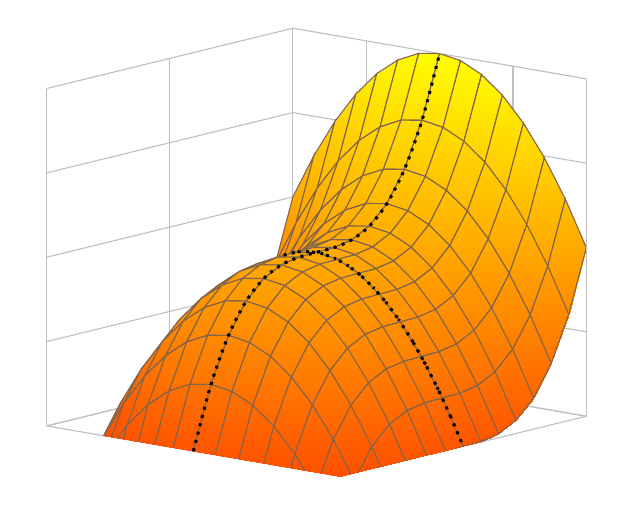
\begin{tikzpicture}
\begin{axis}[xmin=-1.0,xmax=1.0,
             ymin=-1.0,ymax=1.0,
             zmin=-1.0,zmax=1.0,
             grid=major,
             axis line style={draw=none},
             tick style={draw=none},
             view={310}{35},
             xticklabels={\empty},
             yticklabels={\empty},
             zticklabels={\empty},
             plot box ratio={1 1 3},
             colormap/redyellow]
\newcommand\func[2]{#1^3 - #2^2}
\definecolor{darkorange}{HTML}{84644B}

    \addplot3[surf,
              shader=faceted interp,
              faceted color={darkorange},
              samples=15,
              domain=-1:1,
              y domain=-1:1] {\func{x}{y}};

    % plot curve for x direction
    \addplot3[samples=15,
              domain=-1:1,
              samples y=1,
              dotted,
              black,
              line width=1.1pt,
              smooth] (x, 0, \func{x}{0});
    % plot curve for y direction
    \addplot3[samples=15,
              domain=-1:1,
              y domain=-1:0.22,
              dotted,
              black,
              line width=1.1pt,
              smooth] (0, y, \func{0}{y});
\end{axis}
\end{tikzpicture}

        }
        \caption{The principal curvatures are the maximum and minimum \glspl{curvature} in all directions.}\label{fig:curvature_surface}
    \end{subfigure}
    \caption[Curvature of curves and surfaces]{\emph{Curvature of curves and surfaces.} The \gls{curvature} of a curve is defined through its osculating circle. This simple definition is not possible for surfaces in three dimensions. Analyzing all directions, each point on the surface does have a minimum and maximum \gls{curvature} --- the \emph{principal curvatures}.}
\end{figure}
A straight line has no \gls{curvature}, hence $\kappa = 0$.
The \gls{curvature} of a circle is defined is the inverse of its radius
\begin{equation}
    \kappa_{circle} = \frac{1}{r}\text{.}
\end{equation}
Any point's \gls{curvature} on a one-dimensional, twice differentiable function is defined as the \gls{curvature} of its osculating circle, visualized in Figure~\ref{fig:osculating_circle}.
The \gls{curvature} of any point of a surface in three-dimensional space is ambigous, because it has infinite many curves crossing through this point.
But a maximum and minimum \gls{curvature} exist, the \emph{principal curvatures} $k_1$ and $k_2$.
Figure~\ref{fig:curvature_surface} visualizes the directions of the minimum and maximum \gls{curvature} of a surface in three-dimensional space as dotted black lines.
The \emph{\Gls{gaussian-curvature}} $\mathcal{K}$ is defined as the product
\begin{equation}
    \mathcal{K} = k_1 k_2
\end{equation}
and the \emph{\gls{mean-curvature}} $\mathcal{H}$ as the mean
\begin{equation}
    \mathcal{H} = \frac{1}{2} (k_1 k_2)
\end{equation}
of the principal curvatures.

Both quantities can be calculated differently, as the \gls{curvature} is related to the derivates of a function.
Let $f(u, v)$ be a two-dimensional function representing the range image and $f_u$, $f_v$, $f_{uu}$ and $f_{vv}$ its partial derivatives.
Then the \gls{gaussian-curvature} and \gls{mean-curvature} are computed with:
\begin{equation}
\begin{aligned}
    \mathcal{K} &= \frac{f_{uu} f_{vv} - f_{uv}^2}{{(1 + f_u^2 + f_v^2)}^2}\text{,} \\
    \mathcal{H} &= \frac{{(1 + f_{v}^2)} f_{uu} - 2 f_u f_v f_{uv} + {(1 + f_u^2)} f_{vv}}{2 \sqrt{1 + f_u^2 + f_v^2}^3}\text{.}
\end{aligned}
\end{equation}
The central differential quotients approximate the first and second derivatives with $\mathcal{O}(\Delta x^2)$ accuracy:
\begin{equation}
\begin{aligned}
    f_{x} &= \frac{y_{i+1} - y_{i-1}}{2 \Delta x} \\
    f_{xx} &= \frac{y_{i+1} + y_{i-1} - 2 y_{i}}{{\Delta x}^2}\text{.}
\end{aligned}
\end{equation}

\begin{figure}[H]
    \begin{subfigure}[t]{0.32\textwidth}
        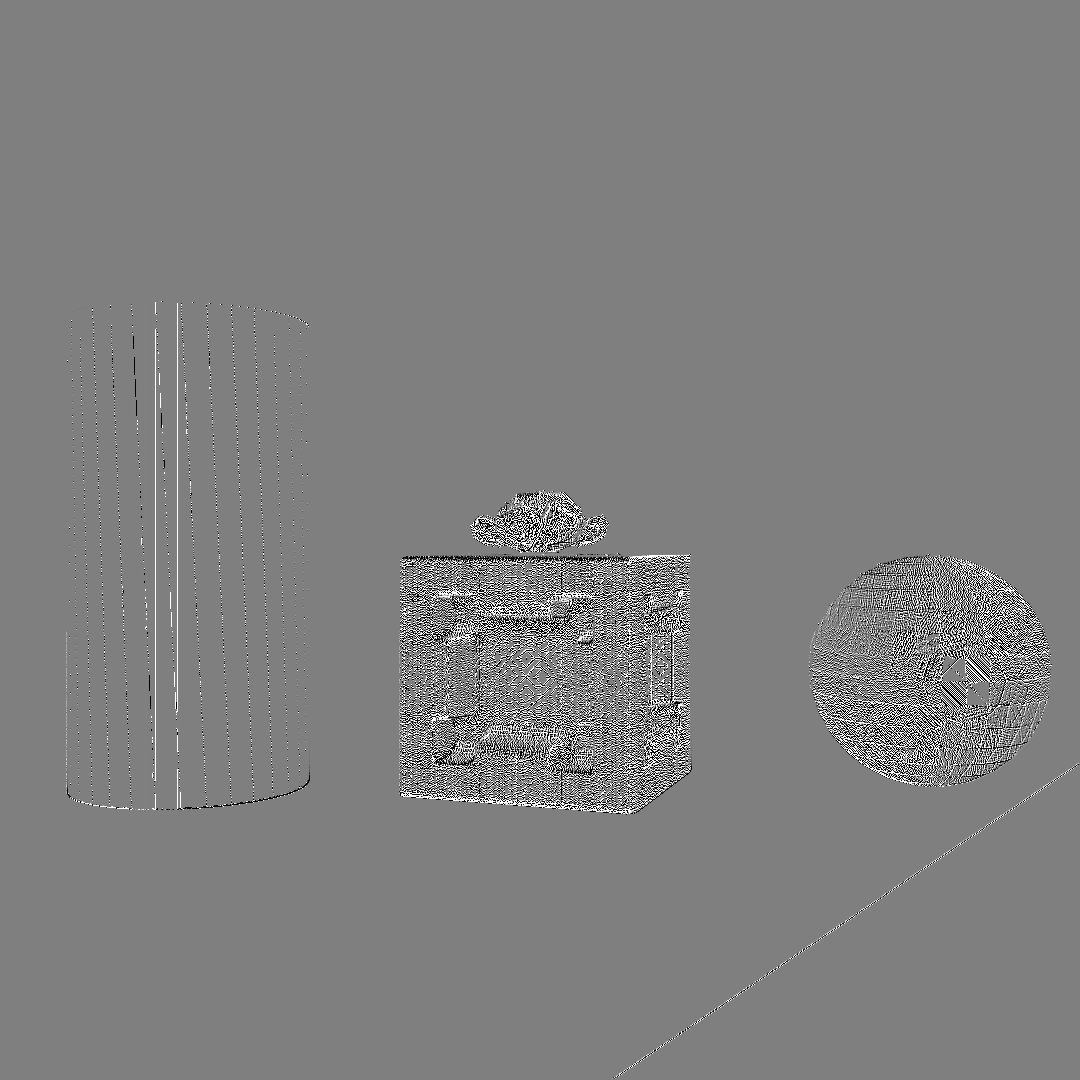
\includegraphics[width=\linewidth]{chapter04/img/mean-0001.png}
    \end{subfigure}
    \begin{subfigure}[t]{0.32\textwidth}
        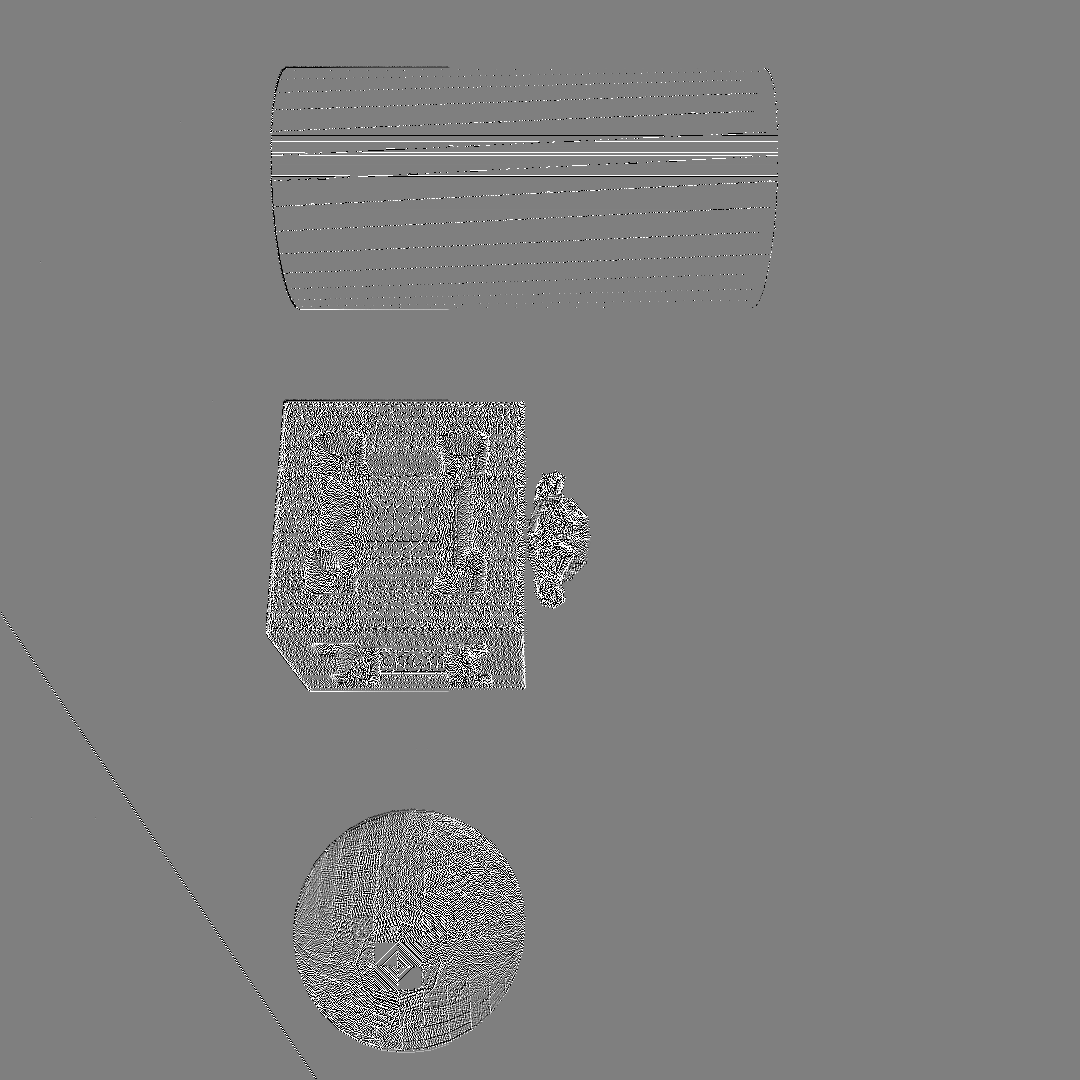
\includegraphics[width=\linewidth]{chapter04/img/mean-0030.png}
    \end{subfigure}
    \begin{subfigure}[t]{0.32\textwidth}
        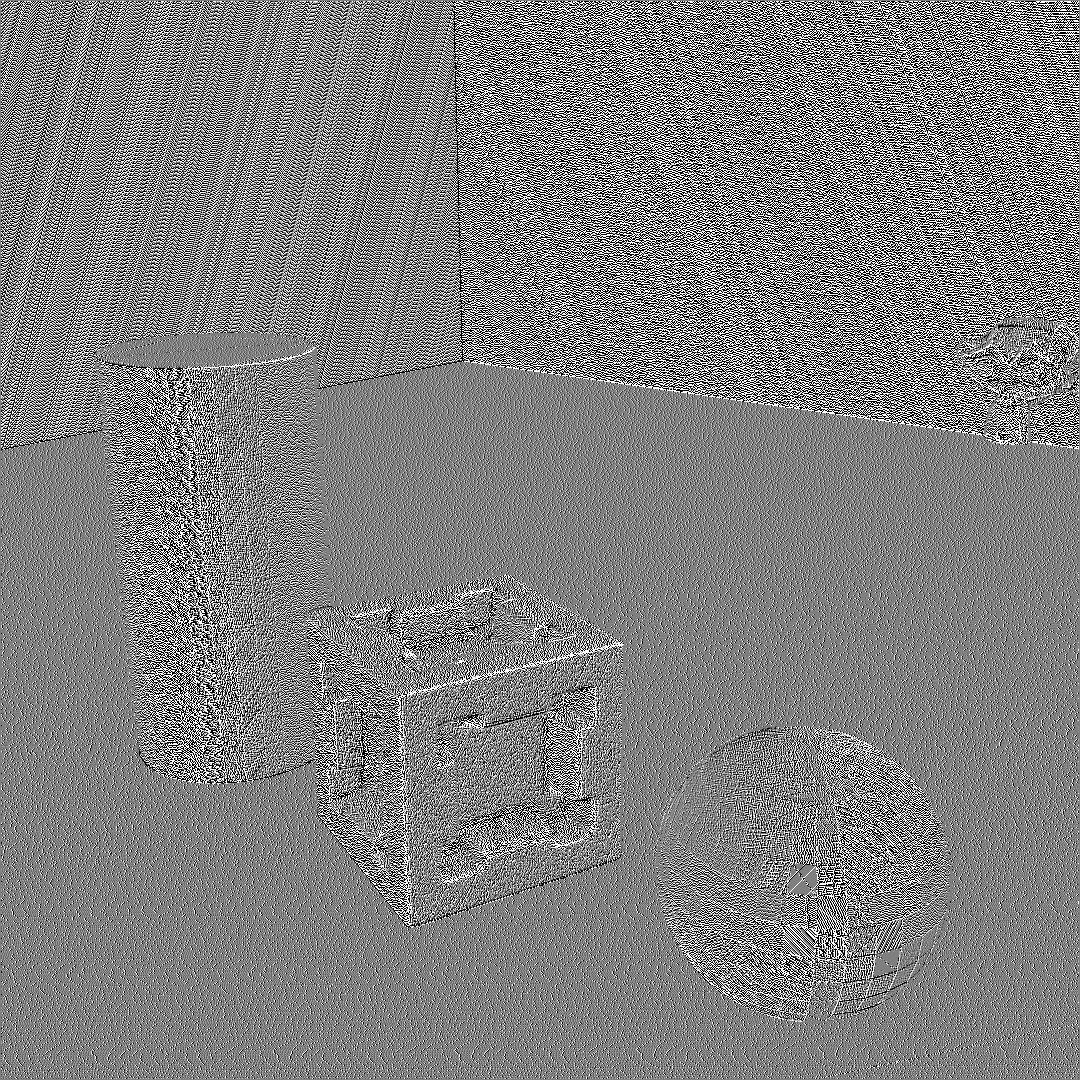
\includegraphics[width=\linewidth]{chapter04/img/mean-0210.png}
    \end{subfigure}
    \caption[\Gls{mean-curvature} in the \emph{Synthetic} scene]{\emph{\gls{mean-curvature} in the Synthetic scene.} The \Gls{mean-curvature} feature image for the same synthetic scene are similar to Multi-Directional \Glspl{bearing-angle-image}, making them a second non-promising option.}\label{fig:mean-curvature}
\end{figure}
The result of the \gls{mean-curvature} conversion in Figure~\ref{fig:mean-curvature} is similar to the Multi-Directional \gls{bearing-angle-image}.
The \gls{mean-curvature} is rotation invariant but the result is already very unstable to the noise induced by integer precision depth images.
Figure~\ref{fig:gaussian-curvature} shows the images for the \gls{gaussian-curvature}.
It is even more prone to noise in the input and suffers from the same range issue.

Both the \gls{mean-curvature} and \gls{gaussian-curvature} are unbound and result in any real number.
Simple scaling between the computed minimum and maximum value is unstable between images and results in completly gray images as these quantities have noticable outliers.
As solution for this problem the computed values are clamped to a predefined range, for example $\mathcal{H},\mathcal{K} \in (-20, 20)$ and then scaled to the desired image depth of the feature image.
\begin{figure}[H]
    \begin{subfigure}[t]{0.32\textwidth}
        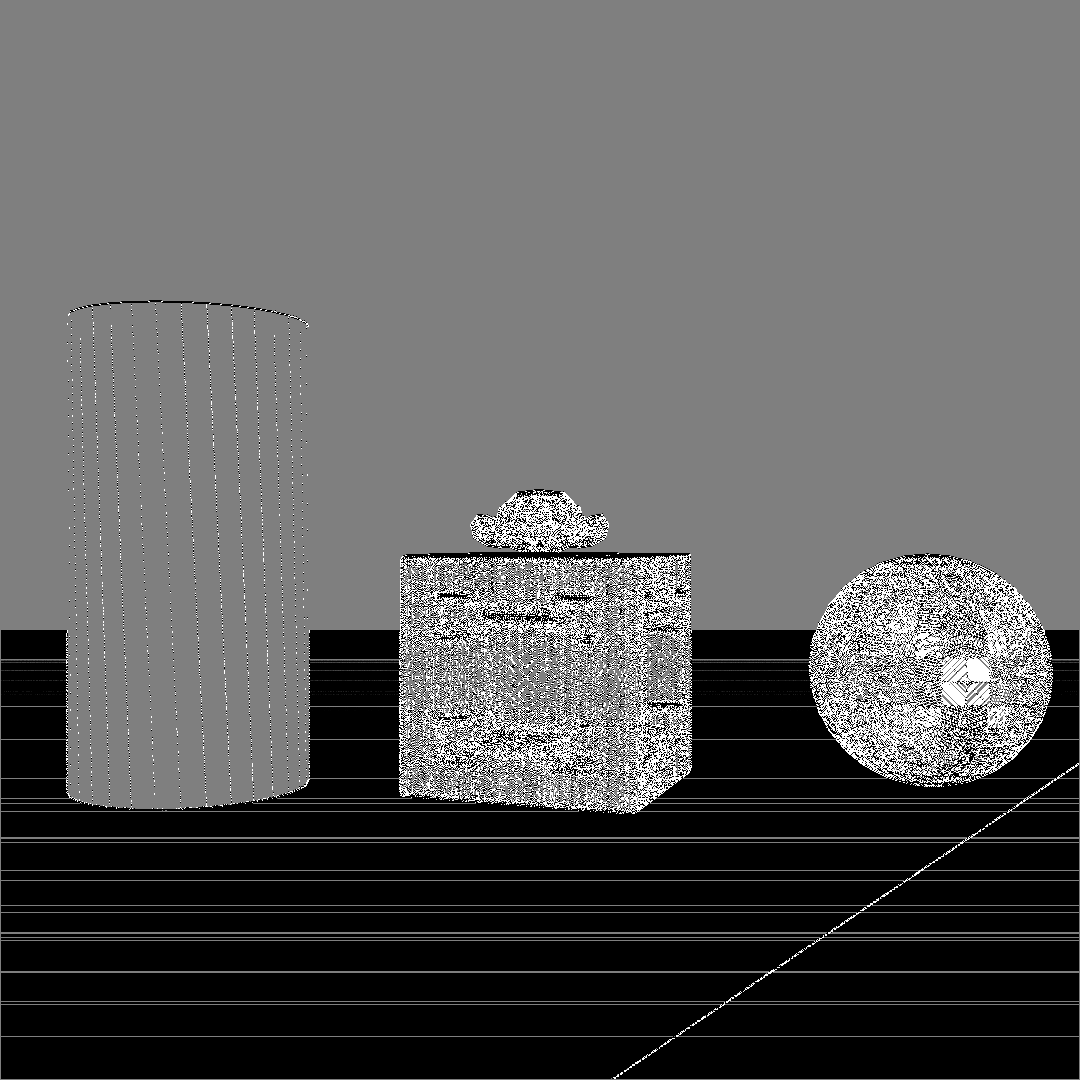
\includegraphics[width=\linewidth]{chapter04/img/gauss-0001.png}
    \end{subfigure}
    \begin{subfigure}[t]{0.32\textwidth}
        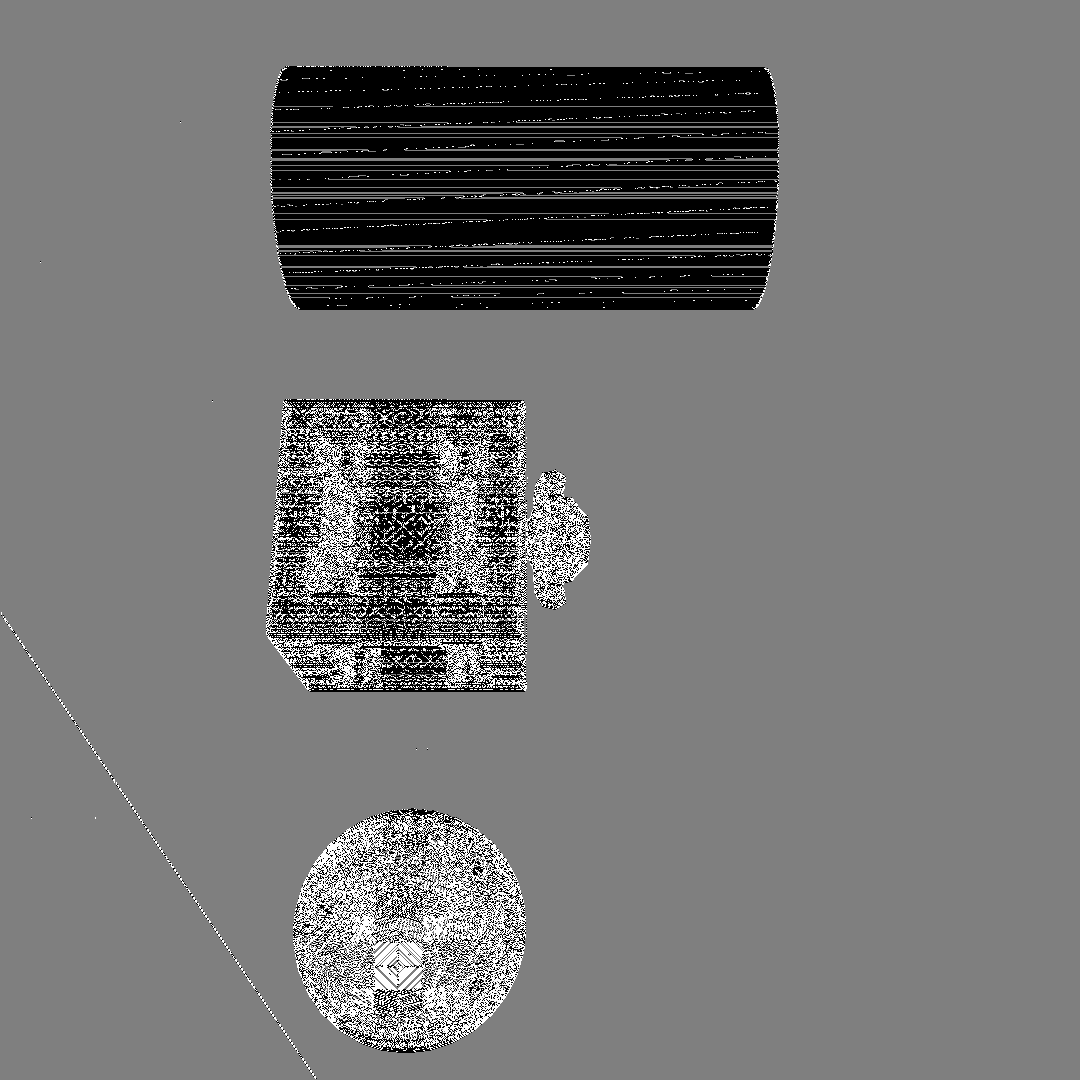
\includegraphics[width=\linewidth]{chapter04/img/gauss-0030.png}
    \end{subfigure}
    \begin{subfigure}[t]{0.32\textwidth}
        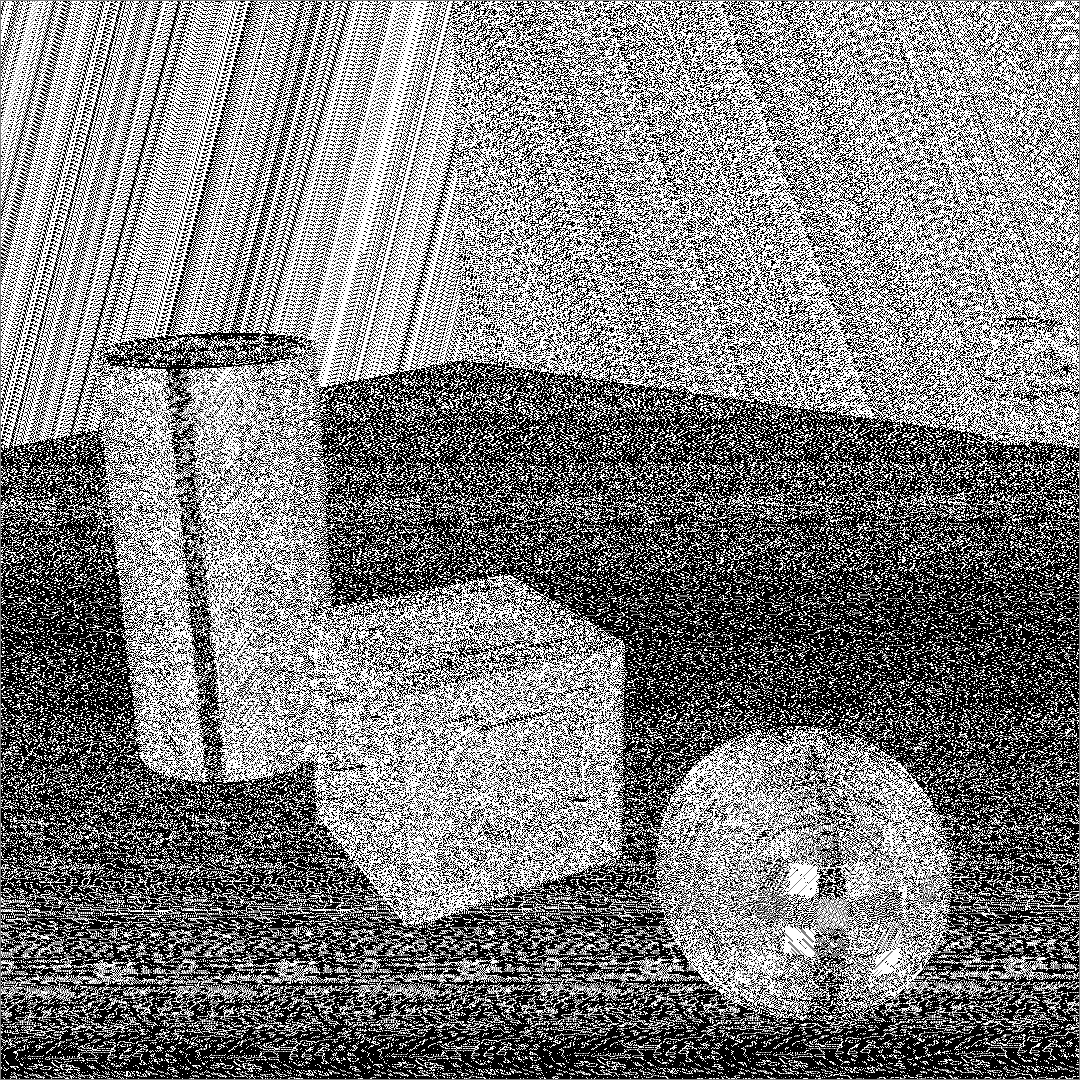
\includegraphics[width=\linewidth]{chapter04/img/gauss-0210.png}
    \end{subfigure}
    \caption[\Gls{gaussian-curvature} in the \emph{Synthetic} scene]{\emph{\Gls{gaussian-curvature} in the Synthetic scene.} The \Gls{gaussian-curvature} feature images for the synthetic scene. The results are not promising either.}\label{fig:gaussian-curvature}
\end{figure}
Computing the curvature for the whole image has the theoretical weakness, that discontinuities at object boundaries are not respected.
The derivatives do not exist at these points for perfect depth sensing.
A mathematically accurate computation requires object identification or meshing of the scene.
Such a requirement seems unreasonable for a foundational processing step in potential real-time use cases.
